\chapter*{CONSTRUCCIÓN DE UNA MONTAÑA RUSA}

\textbf{1)} Un satélite se encuentra en una órbita elíptica alrededor de la Tierra. Su distancia r (en millas) desde el centro de la Tierra está dada por$$r\frac{495}{1+0.12cos\theta}$$

donde $\theta$ es el ángulo medido desde el punto de la órbita más cercano a la superficie de la Tierra (ver la figura adjunta).
\begin{enumerate}[label=\alph*)]
    \item Halla la altitud del satélite en el perigeo (el punto más cercano a la superficie de la Tierra) y en el apogeo (el punto más alejado de la superficie de la Tierra). Usa 3960 mi como el radio de la Tierra.
    \item En el instante en que $\theta$ es 120°, el ángulo $\theta$ aumenta a una tasa de 2,7° /min. Halla la altitud del satélite y la tasa a la que cambia la altitud en ese instante. Expresa la tasa en unidades de mi/min.
\end{enumerate}
\begin{center}
    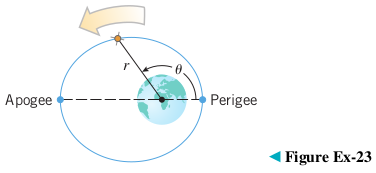
\includegraphics[height = 0.14\textheight]{recursos/image.png}\par
\end{center}

